\documentclass{standalone}
\usepackage{tikz}

\begin{document}

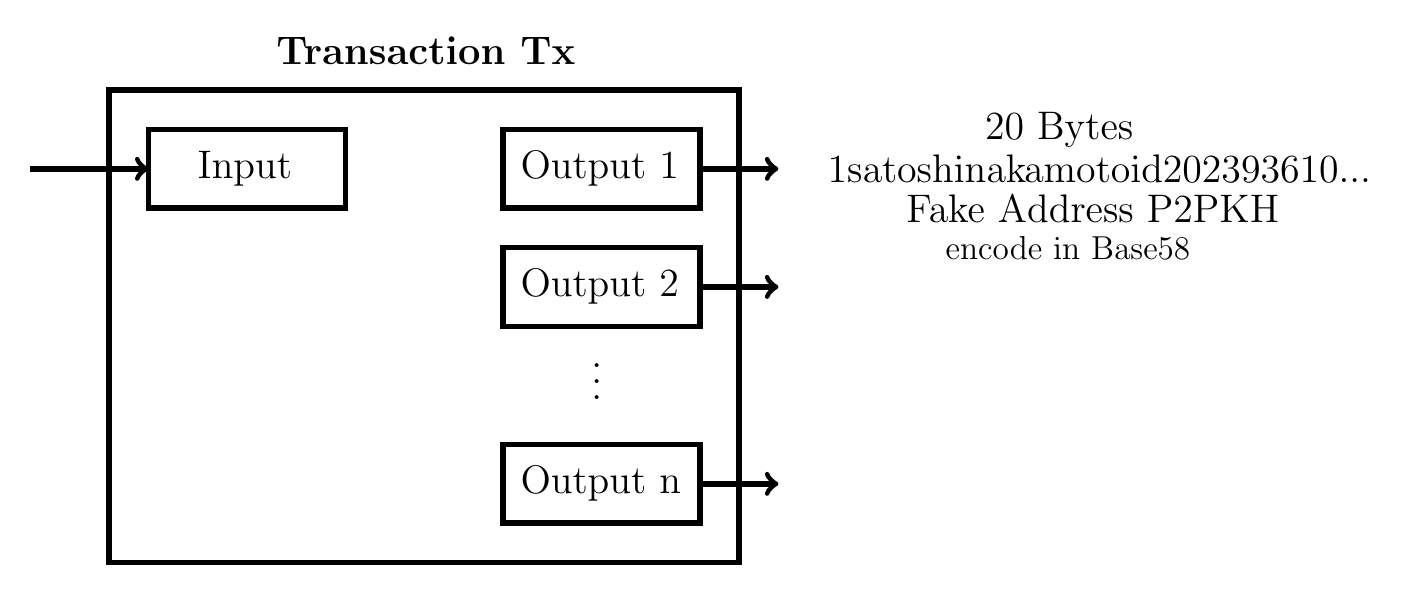
\begin{tikzpicture}
  % \draw[black] (0,1) rectangle (10,9); 
  \draw[line width=2pt] (1,3) rectangle (9,9);

  \draw[line width=2pt] (1.5,8.5) rectangle (4,7.5);
  \draw[line width=2pt] (6,8.5) rectangle (8.5,7.5);
  \draw[line width=2pt] (6,7) rectangle (8.5,6);
  \draw[line width=2pt] (6,4.5) rectangle (8.5,3.5);

  \node[anchor=west, font=\Large] at (2,8) {Input};
  \node[anchor=west, font=\Large] at (6.1,8) {Output  1};
  \node[anchor=west, font=\Large] at (12,8.5) {20 Bytes};
  \node[anchor=west, font=\Large] at (10,8) {1satoshinakamotoid202393610...};
  \node[anchor=west, font=\Large] at (11,7.5) {Fake Address P2PKH};
  \node[anchor=west, font=\large] at (11.5,7) {encode in Base58};
  \node[anchor=west, font=\Large] at (6.1,6.5) {Output 2};
  \node[anchor=west, font=\Large] at (7,5.5) {.};
  \node[anchor=west, font=\Large] at (7,5.3) {.};
  \node[anchor=west, font=\Large] at (7,5.1) {.};
  \node[anchor=west, font=\Large] at (6.1,4) {Output n};
  \node[anchor=west, font=\Large] at (3,9.5) {\textbf{Transaction Tx}};

  \draw[->,line width=2pt] (0,8) -- (1.5,8);
  \draw[->,line width=2pt] (8.5,8) -- (9.5,8);
  \draw[->,line width=2pt] (8.5,6.5) -- (9.5,6.5);
  \draw[->,line width=2pt] (8.5,4) -- (9.5,4);

\end{tikzpicture}

\end{document}
